\documentclass[a4paper, 11pt]{article}
\usepackage{comment} % enables the use of multi-line comments (\ifx \fi) 
\usepackage{fullpage} % changes the margin
\usepackage{graphicx}

\begin{document}

\begin{center}
\textbf{\Large{Network Auto Tester and Evaluator}}\\
\textbf{NATE}
\end{center}

\noindent
\large\textbf{Documentation for V.3.0} \hfill \textbf{by: Andrey G.} \\
\normalsize  \hfill \\
\hfill Generated on: \today 

\tableofcontents
%--------------------------------------------- INTRODUCTION ---------------------------------------------

\section{Network Auto Tester and Evaluator}
Network Auto Tester and Evaluator (NATE) is a framework for automatic training neural networks and evaluating their performance efficiency. The framework allows to design a set of neural network based experiments that will be executed consequently in an automatic manner. Each task allows to specify a neural network architecture, training parameters, datasets, and data augmentation methods - thus allowing to analyze which particular combination of parameters yield the best result in a specific research study. 

The main advantage of the NATE framework is that it frees the user from mundane work of manually launching networks permitting to focus on more important stage of investigation such as network design and result analysis. The standartized procedure of saving intermideate logs, network efficiency measurements and network predictions on a test set also aids with analysis of the results allowing to redo the previous experiments with ease.  

%--------------------------------------------- QUICK LAUNCH ----------------------------------------------

\section{Quick Launch}

\subsection{Build Datasets for Training, Validataion, Testing}
Common dataset loaders implemented in the PyTorch framework operate by scanning the folder structure where image files are located. That is not convenient for 
large datasets with mixed images. Instead of building datasets based on folder structure NATE uses dataset files that provide necessary information about the location
of each sample image and the ground truth vector. 

The format of the dataset files varies depending on the type of task the network will learn to carry out: classification, segmentation, or image encoding. 

\begin{itemize}
\item \textbf{Classification} - each row of the dataset file used in the classification task consists of a path to a sample image\footnote{The path is relative to the image database directory. It is not recommended but possible to use absolute paths, without specifying the "database" path in the task file.} followed by a target N-dimensional vector where elements separated with spaces.

\texttt{row = <path\_to\_image\_file> <n-dimensional vector>}

Example of a row with 5-dim target vector\footnote{See an example file in test/dataset/dataset-cl.txt}: 

\texttt{class1/0030038.png 0 0 1 0 0}

\item \textbf{Segmentation} - the dataset file contains two sections: look up table and paths to image samples and its corresponding map.
The input of the segmentation task is an image, while the output is a segmentation map represented as an image, where different object labels are presented in different colors. The look up table in the dataset file determines the correspondence between a color of an object in the segmentation map and a label index. The label indexes should start from 1 and follow the natural order. Each row of the look up table starts with a key word \textbf{dict:} followed by 3 values that present red, green and blue color and the index of a label. The rows that describe samples are composed of two strings - path to an image and the corresponding segmentation map \footnote{The paths are relative to the image database directory. It is not recommended but possible to use absolute paths, without specifying the "database" path in the task file.}.

\texttt{LUT row = dict: <r> <g> <b> <id>}

\texttt{Sample row = <path\_to\_image\_file> <path\_to\_map\_file>}

Example of a dataset file for segmentation\footnote{See an example file in test/dataset/dataset-seg.txt}:

\texttt{dict: 255 255 255 1}\\
\texttt{dict: 255 255 0 1}\\
\texttt{class1/0030032.png seg/0030032\_seg0.png}\\
\texttt{class1/0030033.png seg/0030033\_seg0.png}\\

\item \textbf{Image encoding} - each row of the dataset file has a path to an input image and path to an output image. The image encoding task is basically an autoencoder.

\texttt{Sample row = <path\_to\_input\_image\_file> <path\_to\_output\_image\_file>}

Example of a dataset row for an autoencoder:

\texttt{class1/0030038.png class1/0030038.png}

\end{itemize}

Depending on the stage of experiments the user desires to carry out it is necessary to generate a number of datasets. For the training only stage (taskstage = train) training and validation sets should be specified. For the testing only stage (task stage = test) a dataset for testing is enough to specify. In case of conducting full loop of training and testing from start-to-end (taskstage = s2e) or resuming the previously terminated start-to-end all three datasets - training, validation, testing - should be generated and specified in the JSON task file.

\subsection{Design Experiments and Create a Task File}
To carry automatic experimentation with different networks and parameters the user has to write the task file in the JSON format. Below an example of such a file is given.

For encoding/decoding type of task the \textbf{network\_classcount} should be set to 3, while for segmentation task the value should be set to the number of segmentation classes.

\begin{verbatim}
{
  "tasklist":
  [
    {
      "tasktype": "class",
      "taskstage": "s2e",
      "taskcheckpoint": "",

      "database": "D:/.../database/",
      "dataset_train": "D:/.../dataset/train.txt",
      "dataset_validate": "D:/.../dataset/validate.txt",
      "dataset_test": "D:/.../dataset/test.txt",

      "output_log": "D:/.../output/log/",
      "output_model": "D:/.../output/model/",
      "output_accuracy": "D:/.../output/score/",

      "network": "densenet121",
      "network_istrained": true,
      "network_classcount": 1,
      "activation": "sigmoid",

      "trnsfrm_train": ["resize", "rndcrop"],
      "trnsfrm_train_param": [256, 224],
      "trnsfrm_validate": ["resize", "rndcrop"],
      "trnsfrm_validate_param": [256, 224],
      "trnsfrm_test": ["resize", "10Crop"],
      "trnsfrm_test_param": [256, 224],

      "loss": "WBCE",
      "epoch": 10,
      "lrate": 0.001,
      "batch": 32
    }
  ]
}
\end{verbatim}

This experiment task will carry start-to-end procedure of training and evaluating a network for solving a binary classification problem. The architecture of the network is DenseNet121 and the initial weights will be assigned from a pre-trained network (ImageNet, torchvision). The loss function used during training procedure is going to be weighted binary cross entropy, learning rate 0.001. The training will be done for 10 epochs with batch size of 32.

To create a new task the user should create a new text file with the formatting described below \footnote{The task file is a JSON file and follows the rules of this format.}.
Each individual task should be specified in the array \texttt{tasklist} surrounded by brackets \{ and \}.

\begin{itemize}
    \item \textbf{tasktype} - defines a type of task that will be carried out. This parameter can have the following string\footnote{Strings in JSON are surrounded by \"!} values: \textbf{class} - for classification task, 
    \textbf{img2img} - for image to image learning (autoencoder), \textbf{seg} - for segmentation task.
    
    \item \textbf{taskstage} - defines what stages of training and testing should be carried out. This parameter can have the following string values: \textbf{train} - for executing only training, \textbf{test} - for executing only testing, \textbf{resume} - for resuming the terminated start-to-end task, \textbf{s2e} - start-to-end task that includes training and testing stages
    
    \item \textbf{taskcheckpoint} - path to the trained model file that can be used for resuming the start-to-end procedure or conducting testing of the trained model. This parameter can be omitted for \textbf{train} and \textbf{s2e} task stages.
    
    \item \textbf{database} - path to the root directory for the image database. Image paths that are written in datasets should be relative to this path.
    
    \item \textbf{dataset\_train} - path to the training dataset file. This setup parameter can be omitted for \textbf{test} task stage.
    
    \item \textbf{dataset\_validate} - path to the validation dataset file. This setup parameter can be omitted for \textbf{test} task stage.
    
    \item \textbf{dataset\_test} - path to the test dataset file. This setup parameter can be omitted for \textbf{train} task stage.
    
    \item \textbf{output\_log} - path to a directory where a log file will be saved.
    
    \item \textbf{output\_model} - path to a directory where a trained network model will be saved.
    
    \item \textbf{output\_accuracy} - path to a directory where the evaluation metrics and results of testing will be saved.
    
    \item \textbf{network} - network architecture. The list of the supported architectures is the following:
    alexnet, convnet12, densenet121, densenet169, densenet201, inception, resnet50, resnet101, vggn16, hrdensenet121, hrdensenet169, scalenet3, fcdensenet103, fcdensenet50 \footnote{See section \ref{nnarch}}
    
    \item \textbf{network\_istrained} - a boolean flag. If set to \textbf{true} then a pre-trained network model is used (for torchvision networks). 
    
    \item \textbf{network\_classcount} - number of output classes if the task is to train a network for a classification or segmentation problems. Should be set up to 3 for image-to-image conversion tasks.
    
    \item \textbf{activation} - type of activation function. Supported only \textbf{sigmoid} and \textbf{softmax} and only for torchvision networks. 
    
    \item \textbf{trnsfrm\_train, trnsfrm\_validate, trnsfrm\_test} - image transformation sequence for the training, validation and test sets. Should be defined as an array and contain one or more (V3.0) transformations: \textbf{resize} - resize and image; \textbf{rndcrop} - random crop; \textbf{ccrop} - center crop; \textbf{10crop} - 10 crop\footnote{10 crop is supported only for testing!}
    
    \item \textbf{trnsfrm\_train\_param, trnsfrm\_validate\_param, trnsfrm\_test\_param} - parameters of the transformation. Should be defined as an array of similar size as the transformations array. The parameters should be specified according to the PyTorch transformation documentation.
	
	\item \textbf{trnsfrm\_seg\_end} - transformation sequence over the labeled maps for the segmentation task
	
	\item \textbf {trnsfrm\_seg\_end\_param} - transfromation sequence parameters for the labeled maps in case of the segmentation task
    
\end{itemize}

\subsection{Laucnh the NATE framework}
It is possible to launch the execution of tasks with the NATE framework by running a script \textbf{runnate.py} with an only required argument being the path 
to the JSON task file.
\newline \newline
\texttt{python runnate.py task-test.json}
\newline \newline
Optional arguments allow to specify if the execution should be done in verbose mode, number of workers for the data loaders and the ID of the gpu to run the execution of the experiments on. Add \textbf{-c} to switch to verbose mode, \textbf{-wc \$number\_of\_workers}\footnote{If running on Windows, set the number of workers to 0, while on LINUX based systems spet to 4-16 depending on the CPU.}, \textbf{-gpu \$gpu\_id}.
\newline \newline
\texttt{python runnate.py task-test.json -c -wc 0 -gpu 0}
\newline \newline

The exution of the task can be initiated using a class \textbf{Nate} from a user defined script.

\begin{verbatim}
import nate as nt

argTaskFile = "task-test.json"
argWorkerCount = 0
argSilentMode = True
argGPU = 0
nt.Nate.run(argTaskFile, argWorkerCount, argSilentMode, argGPU)
\end{verbatim}

\subsection{Check the Processing Stage and Results}
During its execution NATE creats a log file with a name that contains a unique timestamp. The trained model, accuracy scores, predicted data files all share the same timestamp. The generated log file contains information about the launched time and information about the training and validation losses at each epoch. If the trained network achieved better results (lower loss) on a validation test the network model is saved.

After the training stage is completed the network is tested and some measurements for its efficiency are calculated. In case of the classification type of task two files are generated - accuracy and prediction. The accuracy file contains statistics such as AUROC, accuracy, F-score as well as confusion matrix with the number of true positive, false positive, true negative and false negative samples. The prediction file contains the ground truth and the output value for the samples present in the test dataset file. The order of samples is preserved.

For the segmentation and encoding/decoding type of tasks instead of accuracy and prediction files output of the network as images are saved.   

%-------------------------------------- NETWORK ARCHITECTURES ---------------------------------------

\section{Supported Network Architectures}
\label{nnarch}
The following architectures are supported in the NATE framework (V3.0 - Jan 2019).

\begin{itemize}
    \item AlexNet - torchvision implementation of the AlexNet architecture. Input image resolution is 224x224x3, output - N-dimensional vector.
    \item ConvNet12 - a shallow network of 12 convolutions and 6 pooling layers. Input image resolution is 224x224x3, output - N-dimensional vector.
    \item DenseNet121 - torchvision implementation of the DenseNet121 architecture. Input image resolution is 224x224x3, output - N-dimensional vector.
    \item DenseNet169 - torchvision implementation of the DenseNet169 architecture. Input image resolution is 224x224x3, output - N-dimensional vector.
    \item DenseNet201 - torchvision implementation of the DenseNet169 architecture. Input image resolution is 224x224x3, output - N-dimensional vector.
    \item Inception - torchvision implementation of the Inception architecture. Input image resolution is 224x224x3, output - N-dimensional vector.
    \item ResNet50 - torchvision implementation of the RenseNet50 architecture. Input image resolution is 224x224x3, output - N-dimensional vector.
    \item ResNet101 - torchvision implementation of the RenseNet101 architecture. Input image resolution is 224x224x3, output - N-dimensional vector.
    \item VGGN16 - torchvision implementation of the RenseNet101 architecture. Input image resolution is 224x224x3, output - N-dimensional vector.
    \item HRDenseNet121 - a DenseNet121 network which allows to supply 3-channel images of any resolution, output is an N-dimensional vector. 
    \item HRDenseNet169 - a DenseNet169 network which allows to supply 3-channel images of any resolution, output is an N-dimensional vector. 
    \item ScaleNet3 - a shallow architecture which contcatenates feature maps on different scales. Input image resolution is 227x227x3, output is an N-dimensional vector.
    \item FcDenseNet103 - DenseNet Teramisu (FC-DenseNet) with 103 layers. This network can be used for autoencoder tasks or segmentation. Any sensible resolution is supported for the input, but the input should have 3 channels. The output is the same resolution as the input, with N channels.
    \item FcDenseNet50 - DenseNet Teramisu (FC-DenseNet) with 50 layers. This network can be used for autoencoder tasks or segmentation. Any sensible resolution is supported for the input, but the input should have 3 channels. The output is the same resolution as the input, with N channels.

\end{itemize}

\begin{figure}
    \centering
    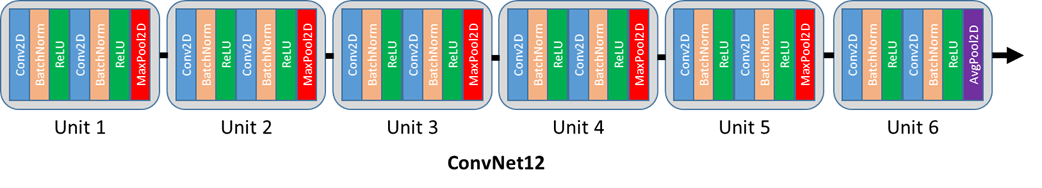
\includegraphics[width=0.8\textwidth]{img/convnet12.png}
    \caption{Architectuer of the ConvNet12 network}
    \label{convnet12}
\end{figure}


\section{Detail Description of the Task File}
A more detailed description of the parameters that can be found in a task file a presented in the Table \ref{tabjson}.

Pay attention that for the encoding/decoding type of task the network\_classcount should be set to 3. In case of the segmentation task, this parameter has to be specified as the number of labels in the segmentation maps.

Some parameters are mandatory and should be defined in evert task file, while others are optional and require definition only for a specific task stages (training, testing, start-to-end or resume) or task types. Particular, the transformation that affects the output segmentation map of the segmentation task is required to be defined for that particular task only. It can be ommited in other task types. Nevertheless, it is recommended to leave the parameters and set the particular value to
0 or empty string.

\begin{center}
\begin{table}
\label{tabjson}
\begin{tabular}{|l|l|l|l|}
\hline
PARAMETER & VALUE & MANDATORY  \\
\hline
tasktype & \textbf{class} - classification & YES \\
		 & \textbf{seg} - segmentation &  \\
		 & \textbf{img2img} - image encoding & \\
\hline
taskstage & \textbf{train} - training & YES \\
		  & \textbf{test} - testing & \\
		  & \textbf{s2e} - traing then testing & \\
		  & \textbf{resume} - training then testing & \\
\hline
taskcheckpoint & absolute path & taskstage = test, resume \\ 
\hline
database & absolute path & YES \\
\hline
dataset\_train & absolute path & taskstage = train, s2e, resume \\
\hline
dataset\_validate & absolute path &  taskstage = train, s2e, resume\\
\hline
dataset\_test & absolute path &  YES  \\
\hline
output\_log & absolute path & taskstage = train, s2e, resume  \\
\hline
output\_model & absolute path & taskstage = train, s2e, resume \\
\hline
output\_accuracy & absolute path & YES for any taskstage \\
\hline
network & alexnet, convnet12, densenet121,& YES \\
&  densenet169, densenet201, inception,  & \\
& resnet50, resnet101, vggn16, scalenet3,  &\\
& hrdensenet169,  fcdensenet103,  &\\
& fcdensenet50, hrdensenet121 & \\
\hline 
network\_istrained & true, false & YES \\
\hline 
network\_classcount & integer, 3 for img2img  & YES \\
\hline 
activation & sigmoid, softmax & YES \\
\hline 
trnsfrm\_train & array: resize, ccrop, rndcrop & taskstage = train, s2e, resume \\
trnsfrm\_train\_param & array: integers & \\
\hline 
trnsfrm\_validate & array: resize, ccrop, rndcrop & taskstage = train, s2e, resume \\
trnsfrm\_validate\_param & array: integers & \\
\hline 
trnsfrm\_test & array: resize, ccrop, rndcrop, 10crop & taskstage = test, resume \\
trnsfrm\_test\_param & array: integers & \\
\hline 
trnsfrm\_set\_end & array: resize, ccrop & tasktype = seg \\
trnsfrm\_seg\_end\_param & array: integers & \\
\hline
loss & BCE, WBCE, WBCEMC, MSE & taskstage = train, s2e, resume \\
\hline
epoch & integer & taskstage = train, s2e, resume \\
\hline 
lrate & double & taskstage = train, s2e, resume \\
\hline 
batch & integer & YES\\
\hline 
\end{tabular}
\caption{Possible combination of parameters of the task file.}
\end{table}
\end{center}


\section{Internal Architecture}
This section contains description of the internal architecture of the NATE framework and several tips on implementing new functionaslity.

%--------------------------------------------- WORKFLOW ---------------------------------------------
\subsection{Core Workflow of the Sytem}
The execution of the set of tasks specified in a JSON file is split into several stages. First the JSON is parsed and for each task a separated object that holds textural description of the task - \textbf{TaskSettings} - is created\footnote{Preliminary correctness checks are also done during JSON parsing}. 
These objects are gathered together in a list \textbf{TaskSettingsCollection}. Then the script enters the main procedural loop. It picks one task from the list of tasks and generates an execution environment checking the correctness of provided data \textbf{TaskEnvironment}. At the generation stage the network model, data loaders are created and file system environment variables are instantiated. The generation step is followed by execution stage where NATE carries out training and testing procedures. In the following sections detailed description of classes and modules is given.
\begin{figure}
    \centering
    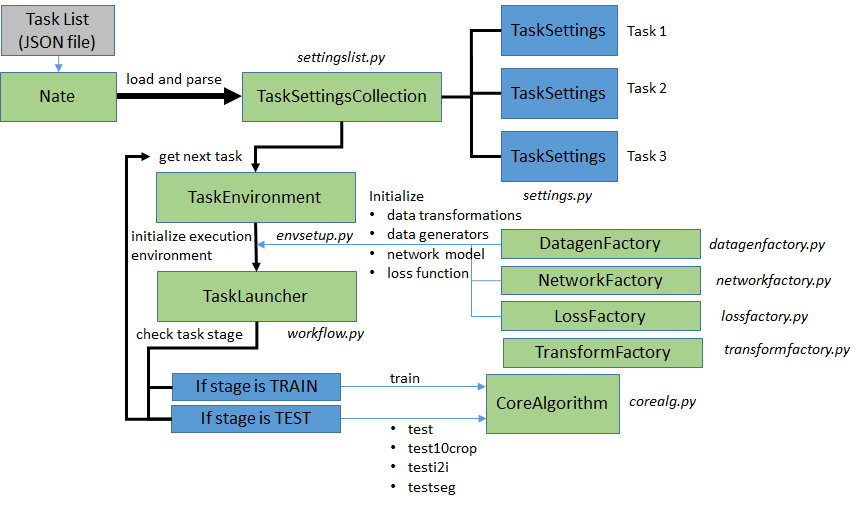
\includegraphics[width=0.8\textwidth]{img/schemenate1.png} 
    \caption{Workflow of the NATE training and testing procedure. At the first step the input JSON file is loaded with the class TaskSettingsCollection that creates a list of tasks consisting of objects TaskSettings. Next the necessary execution environment is initialized by generating necessary model, loss, data generators and other necessary objects using a number of factory classes. The execution is than handled to TaskLauncher class, that prepares specifies the environment for each stage of the task: training or testing. The immediated iteration through epochs and testing procedures are carried out then by CoreAlgorithm class.}
    \label{fig:my_label}
\end{figure}

\subsection{Modules, Files and Classes}
\begin{center}
\begin{table}[h]
\begin{tabular}{l|l|l}
	\hline
	MODULE & FILE & CLASSES \\
	\hline
	datagen & classification.py & DatagenClassification \\
	datagen & segmentation.py &  DatagenSegmentation, DatagenAutoencoder \\
	datagen & datagenfactory.py & DatagenFactory \\
	\hline
	loss & lossfactory.py & LossFactory\\
	loss & losszoo & WeightedBinaryCrossEntropyMC, WeightedBinaryCrossEntropy\\
	\hline
	network & alexnet.py & AlexNet \\
	network & convnet.py &  ConvNet12\\
	network & densenet.py & DenseNet121, DenseNet169, DenseNet201, \\
	& & HRDenseNet121, HRDenseNet169\\
	netowrk & fcwdensenet.py & FCWDenseNet103, FCWDenseNet50 \\
	netwrok & inceptionnet.py &  Inception\\
	netwrok & resnet.py & ResNet50, ResNet101\\
	netwrok & scalenet.py & ScaleNet3\\
	netwrok & vggnet.py & VGGN16\\
	netwrok & netfactory.py & NetworkFactory\\
	\hline
	score & judge.py & ScoreCalculator\\
	\hline 
	settings & settings.py & TaskSettings \\
	settings & settingslist.py & TaskSettingsCollection \\
	\hline
	transform & transformfactory.py & TransformFactory \\
	\hline 
	nate & corealg.py &  CoreAlgorithm \\
	nate & corenate.py & Nate \\
	nate & envsetup.py & TaskEnvironment \\
	nate & workflow.py & TaskLauncher \\
	\hline
	
\end{tabular}
\caption{A table of classes and files where they could be found}
\end{table}
\end{center}

%--------------------------------------------- MODULES ---------------------------------------------
\subsection{Modules}
The NATE framework is split into following separated modules
\begin{itemize}
    \item \textbf{datagen} (nate/datagen) - data generators and a factory for generating specific data generators
    \item \textbf{loss} (nate/loss) - a collection of custom loss functions and a factory class that returns a specific instance of a loss function by its name
    \item \textbf{network} (nate/network) - a collection of network classes and a factory for generating a particular network by specifying its name and additional parameters
    \item \textbf{score} (nate/score) - methods for evaluating the efficiency of the trained network (AUROC, F-score, Precision Recall etc)
    \item \textbf{settings} (nate/settings) - classes that describe parameters of an individual and multiple tasks
    \item \textbf{transform} (nate/transform) - a factory for initializing transfromations for data augmentations
\end{itemize}

There are also a number of scrips that implement the core functionality of the NATE framework: \textit{corealg.py}, \textit{corenate.py}, \textit{envsetup.py}, \textit{workflow.py}.

\subsubsection{Module: datagen} 
This module contains data generator classes. They are respondible for processing the dataset files and converting in a format understandable by the PyTorch framework. 
Each data generator class derived from a PyTorch generator class \textbf{Dataset}. To ease the usage of datagenerators a factory class is implemented. 

\subsubsection{Module: loss}
There are a few loss functions that are currently supported by the system. It is possible to implement additional custom loss functions or add those supported by PyTorch framework. Check section \ref{myloss} for more details.
\subsubsection{Module: network}
Module network\footnote{Located in nate/network} contains python files that contains classes describing neural network architectures and contains an implementation of the network factory class \textbf{NetworkFactory}\footnote{See file netfactory.py}
\subsubsection{Module: score}
This module contains classes and method for measuring the efficiency of the trained network. The core class ScoreCalculator allows to get AUROC, F-score, confusin matrix data. In case of multi-class classification problem individual statistics are calculated for each class and stored in the accuracy class after testing is finished. 
\subsubsection{Module: settings}
This module contains classes that store information loaded from a task file.
\subsubsection{Module: transform}
Module where various transformations are implemented. For the segmentation task it was necessary to define a separate transformation methods to prevent loss of data due to interpolation method of the Resize transfromation.

%---------------------------------------- CHANGING THE CORE ----------------------------------------
\section{Adding Functionality}

\subsection{I want to add a new network architecture for an existing type of task}
Existing types of tasks are: classification, segmentation and image encoding/decoding.

\begin{enumerate}
\item Implement a network class deriving the PyTorch \textit{nn.Module} with the mandatory methods of \textit{forward} [PyTorch forward pass], \textit{getsizein} [should return the size of the input tensor as an array], \textit{getsizeout} [should return the size of the output tensor as an array].
\item Add a new network name into the \textbf{NETWORK\_TABLE} dictionary of the \textbf{NetworkFactory} class, change the \textbf{getNetwork} method.
\end{enumerate}

\subsection{I want to add a new transformation for data augmentation}
Supported transformation in this versions do vary for training, validation and tests sets and different tasks.

\begin{itemize}
\item Classification 
	\begin{itemize}
	\item Training, Validataion: Random resized crop, Resize, CenterCrop 
	\item Testing: Random resized crop, Resize, CenterCrop, 10Crop
	\end{itemize}
\item Segmentation
	\begin{itemize}
	\item Training, Validation, Testing input image: Random resized crop, Resize, CenterCrop 
	\item Training, Validation, Testing output image: Random resized crop (interpolation=Nearest neighbor), Resize (interpolation=Nearest neighbor), CenterCrop 
	\end{itemize}
\item Encoding and Decoding
	\begin{itemize}
	\item Training, Validataion input image and output image: Random resized crop, Resize, CenterCrop 
	\item Testing input image and output image: Random resized crop, Resize, CenterCrop
	\end{itemize}
\end{itemize}

It has to be noted that random transformation for segmentation and encoding tasks should be tackled with extreme carefullness. Since the random parameters of the transformation for input sample and output sample could be different for correct allignment the random generators should be initialized with a similar seed.

Follow the steps below to add a new transformation procedure.
\begin{enumerate}
\item Add a new transformation to the \textbf{TRANSFORM\_TABLE} of the \textbf{TransformFactory} class. Update the \textbf{getTransformSequence} method or implement your own.
\item If it is a completely new method for generation of the transformation sequence, the class \textbf{TaskEnvironment} should be updated. In some cases it will be also necessary to update the training or testing procedure of the \textbf{TaskLauncher} class.
\end{enumerate}

\subsection{I want to add a new loss function}
\label{myloss}
\begin{enumerate}
\item Implement your new custom loss function. It is recommended to implement it in the file \textbf{losszoo.py}. 
\item Add the name of the loss function to the \textbf{LossFactory} and update the method \textbf{getLossFunction}.
\end{enumerate}

\subsection{I want to add a custom data generator}
\begin{enumerate}
\item Implement your custom datagenerator class. It should be derived from the \textbf{torch.utils.data.Dataset} class. Use the existing data generators as a reference. 
It is recommended to implement the method \textbf{getfrequency} to preserve compatibility.
\item Add the new data generator to the factory class \textbf{DatagenFactory} and update the \textbf{getDatagen} method.
\end{enumerate}

\subsection{I want to add a new measurement for evaluating network efficiency}
Depending on the aim the difficulty of adding new methods would vary. General recommendations are the following.
\begin{enumerate}
\item Check the \textbf{score/judge.py} file where methods for evaluating the trained networks are stored. 
\item Update or re-implement the testing procedures that are found in the class \textbf{CoreAlgorithm}
\end{enumerate}

\subsection{I want to change the structure of the log file, output file}
\begin{itemize}
\item The header of the log file is stored during executing the \textbf{launch(...)} method of the \textbf{TaskLauncher} class
\item The real-time information about the training and validation losses are done in the \textbf{train} method of the \textbf{CoreAlgorithm}
\end{itemize}

\end{document}
